\documentclass[MAIN.tex]{subfiles}
\begin{document}

\subsection{Alternative agreement indices}
As an alternative to limits of agreement, \citet{lin2002} proposes the use of
the mean square deviation is assessing agreement. The mean square
deviation is defined as the expectation of the squared differences
of two readings . The MSD is usually used for the case of two
measurement methods $X$ and $Y$ , each making one measurement for
the same subject, and is given by
\[
MSDxy = E[(x - y)^2]  = (\mu_{x} - \mu_{y})^2 + (\sigma_{x} -
\sigma_{y})^2 + 2\sigma_{x}\sigma_{y}(1-\rho_{xy}).
\]


\citet{Barnhart} advises the use of a predetermined upper limit
for the MSD value, $MSD_{ul}$, to define satisfactory agreement.
However, a satisfactory upper limit may not be properly
determinable, thus creating a drawback to this methodology.


\citet{Barnhart} proposes both the use of the square root of the
MSD or the expected absolute difference (EAD) as an alternative agreement indices. Both of these indices can be interpreted intuitively, being denominated in the same units of measurements as the original
measurements. Also they can be compare to the maximum acceptable
absolute difference between two methods of measurement $d_{0}$.
\[
EAD = E(|x - y|) = \frac{\sum |x_{i}- y_{i}|}{n}
\]

The EAD can be used to supplement the inter-method bias in an
initial comparison study, as the EAD is informative as a measure
of dispersion, is easy to calculate and requires no distributional
assumptions.

\citet{Barnhart} remarks that a comparison of EAD and MSD , using
simulation studies, would be interesting, while further adding
that `It will be of interest to investigate the benefits of these
possible new unscaled agreement indices'. For the Grubbs' `F vs C' and `F vs T' comparisons, the inter-method bias, difference variances, limits of agreement and EADs are shown
in Table 1.5. The corresponding Bland-Altman plots for `F vs C' and `F vs T' comparisons were depicted previously on Figure 1.3. While the inter-method bias for the `F vs T' comparison is smaller, the EAD penalizes the comparison for having a greater variance of differences. Hence the EAD values for both comparisons are much closer.
\begin{table}[ht]
	\begin{center}
		\begin{tabular}{|c|c|c|}
			\hline
			& F vs C & F vs T  \\
			\hline
			Inter-method bias & -0.61 & 0.12 3 \\
			Difference variances & 0.06 & 0.22  \\
			Limits of agreement & (-1.08,	-0.13) & (-0.81,1.04) \\
			EAD & 0.61 & 0.35  \\
			\hline
		\end{tabular}
		\caption{Agreement indices for Grubbs' data comparisons.}
	\end{center}
\end{table}

Further to  \citet{lin2000} and \citet{lin2002}, individual agreement between two measurement methods may be
assessed using the the coverage probability (CP) criteria or the total deviation index (TDI). If $d_{0}$ is predetermined as the maximum acceptable absolute difference between two methods of measurement, the probability that the absolute difference of two measures being less than $d_{0}$ can be computed. This is known as the coverage probability (CP).

\begin{equation}
CP = P(|x_{i} - y_{i}| \leq d_{0})
\end{equation}

If $\pi_{0}$ is set as the predetermined coverage probability, the
boundary under which the proportion of absolute differences is
$\pi_{0}$ may be determined. This boundary is known as the `total
deviation index' (TDI). Hence the TDI is the $100\pi_{0}$
percentile of the absolute difference of paired observations.

	\section{Alternative agreement indices}
	As an alternative to limits of agreement, \citet{lin2002} proposes the use of the mean square deviation is assessing agreement. The mean square deviation is defined as the expectation of the squared differences	of two readings. 
	
	The MSD is usually used for the case of two
	measurement methods $X$ and $Y$ , each making one measurement for	the same subject, and is given by
	\[
	MSDxy = E[(x - y)^2]  = (\mu_{x} - \mu_{y})^2 + (\sigma_{x} -
	\sigma_{y})^2 + 2\sigma_{x}\sigma_{y}(1-\rho_{xy}).
	\]
	
	
	\citet{Barnhart} advises the use of a predetermined upper limit
	for the MSD value, $MSD_{ul}$, to define satisfactory agreement.
	However, a satisfactory upper limit may not be properly
	determinable, thus creating a drawback to this methodology.
	
	
	\citet{Barnhart} proposes both the use of the square root of the
	MSD or the expected absolute difference (EAD) as an alternative agreement indices. Both of these indices can be interpreted intuitively, being denominated in the same units of measurements as the original
	measurements. Also they can be compare to the maximum acceptable
	absolute difference between two methods of measurement $d_{0}$.
	\[
	EAD = E(|x - y|) = \frac{\sum |x_{i}- y_{i}|}{n}
	\]
	
	The EAD can be used to supplement the inter-method bias in an
	initial comparison study, as the EAD is informative as a measure
	of dispersion, is easy to calculate and requires no distributional
	assumptions.
	
	\citet{Barnhart} remarks that a comparison of EAD and MSD , using
	simulation studies, would be interesting, while further adding
	that `\textit{It will be of interest to investigate the benefits of these
		possible new unscaled agreement indices}'. For the Grubbs' `F vs C' and `F vs T' comparisons, the inter-method bias, difference variances, limits of agreement and EADs are shown
	in Table 1.5. The corresponding Bland-Altman plots for `F vs C' and `F vs T' comparisons were depicted previously on Figure 1.3. While the inter-method bias for the `F vs T' comparison is smaller, the EAD penalizes the comparison for having a greater variance of differences. Hence the EAD values for both comparisons are much closer.
	\begin{table}[ht]
		\begin{center}
			\begin{tabular}{|c|c|c|}
				\hline
				& F vs C & F vs T  \\
				\hline
				Inter-method bias & -0.61 & 0.12 3 \\
				Difference variances & 0.06 & 0.22  \\
				Limits of agreement & (-1.08,	-0.13) & (-0.81,1.04) \\
				EAD & 0.61 & 0.35  \\
				\hline
			\end{tabular}
			\caption{Agreement indices for Grubbs' data comparisons.}
		\end{center}
	\end{table}
	
	Further to  \citet{lin2000} and \citet{lin2002}, individual agreement between two measurement methods may be
	assessed using the the coverage probability (CP) criteria or the total deviation index (TDI). If $d_{0}$ is predetermined as the maximum acceptable absolute difference between two methods of measurement, the probability that the absolute difference of two measures being less than $d_{0}$ can be computed. This is known as the coverage probability (CP).
	
	\begin{equation}
	CP = P(|x_{i} - y_{i}| \leq d_{0})
	\end{equation}
	
	If $\pi_{0}$ is set as the predetermined coverage probability, the
	boundary under which the proportion of absolute differences is
	$\pi_{0}$ may be determined. This boundary is known as the `total
	deviation index' (TDI). Hence the TDI is the $100\pi_{0}$
	percentile of the absolute difference of paired observations.
	
	

\section{Alternative Agreement Indices}
As an alternative to limits of agreement, \citet{lin2002} proposes the use of
the mean square deviation in assessing agreement. The mean square
deviation is defined as the expectation of the squared differences
of two readings. The MSD is usually used for the case of two
measurement methods $X$ and $Y$, each making one measurement for
the same subject, and is given by
\[
MSDxy = E[(x - y)^2]  = (\mu_{x} - \mu_{y})^2 + (\sigma_{x} -
\sigma_{y})^2 + 2\sigma_{x}\sigma_{y}(1-\rho_{xy}).
\]


\citet{Barnhart} advises the use of a predetermined upper limit
for the MSD value, $MSD_{ul}$, to define satisfactory agreement.
However, a satisfactory upper limit may not be easily
determinable, thus creating a drawback to this methodology.


Alternative indices, proposed by \citet{Barnhart}, are the square root of the MSD and the expected absolute difference (EAD). 
\[
EAD = E(|x - y|) = \frac{\sum |x_{i}- y_{i}|}{n}
\]


Both of these indices can be interpreted intuitively, since their units are the same as that of the original
measurements. Also they can be compared to the maximum acceptable
absolute difference between two methods of measurement $d_{0}$. 

The EAD can be used to supplement the inter-method bias in an
initial comparison study, as the EAD is informative as a measure
of dispersion, is easy to calculate and requires no distributional
assumptions. A consequence of using absolute differences is that high variances would result in a higher EAD value. 

% latex table generated in R 3.1.1 by xtable 1.7-4 package
% Mon Feb 23 21:12:33 2015
% latex table generated in R 3.1.1 by xtable 1.7-4 package
% Mon Feb 23 21:13:45 2015
% latex table generated in R 3.1.1 by xtable 1.7-4 package
% Mon Feb 23 22:10:26 2015
\begin{table}[ht]
	\centering
	\begin{tabular}{rrrrr}
		\hline
		& X & Y & U & V \\ 
		\hline
		1 & 101.83 & 102.52 & 98.05 & 99.53 \\ 
		2 & 101.68 & 102.69 & 99.17 & 96.53 \\ 
		3 & 97.89 & 99.01 & 100.31 & 97.55 \\ 
		4 & 98.15 & 99.57 & 100.35 & 96.03 \\ 
		5 & 99.94 & 100.85 & 99.51 & 99.00 \\ 
		6 & 98.85 & 98.86 & 98.50 & 100.76 \\ 
		7 & 99.86 & 97.85 & 100.66 & 99.37 \\ 
		8 & 101.57 & 100.21 & 99.66 & 108.87 \\ 
		9 & 100.12 & 99.85 & 99.70 & 105.16 \\ 
		10 & 99.49 & 98.77 & 101.55 & 94.31 \\ 
		\hline
	\end{tabular}
\end{table}


\begin{verbatim}

Differences  2.5% limit 97.5% limit    SD(diff) 
-0.08078844 -2.39471014  2.23313327  1.15696085 
\end{verbatim}

\begin{table}[ht]
	\centering
	\begin{tabular}{|c|c|c|c|c|}
		\hline
		& X & Y & $X-Y$ & $|X-Y|$ \\ 
		\hline
		1 & 98.05 & 99.53 & -1.49 & 1.49 \\ 
		2 & 99.17 & 96.53 & 2.64 & 2.64 \\ 
		3 & 100.31 & 97.55 & 2.75 & 2.75 \\ 
		4 & 100.35 & 96.03 & 4.32 & 4.32 \\ 
		5 & 99.51 & 99.00 & 0.51 & 0.51 \\ 
		6 & 98.50 & 100.76 & -2.26 & 2.26 \\ 
		7 & 100.66 & 99.37 & 1.29 & 1.29 \\ 
		8 & 99.66 & 108.87 & -9.21 & 9.21 \\ 
		9 & 99.70 & 105.16 & -5.45 & 5.45 \\ 
		10 & 101.55 & 94.31 & 7.24 & 7.24 \\ 
		\hline
	\end{tabular}
	\caption{Example data set}
	\label{EADdata}
\end{table}

To illustrate the use of EAD, consider table ~\ref{EADdata}. The inter-method bias is 0.03, which is quite close to zero, and conducive to agreement between methods. However, an identity plot would indicate very poor agreement, as the points are noticeably distant from the line of equality.
\begin{figure}
	\centering
	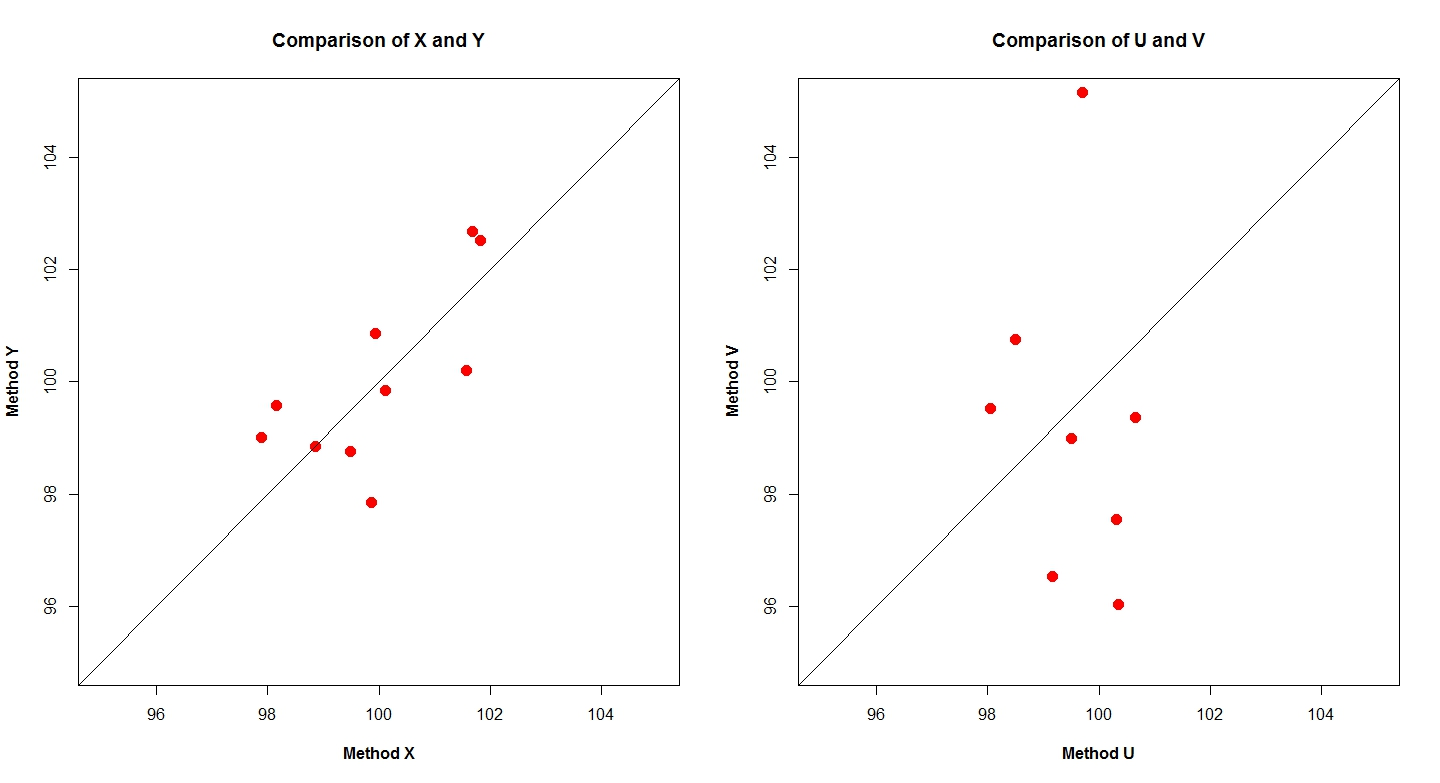
\includegraphics[width=0.7\linewidth]{images/EADidentity}
	\caption{Identity Plot for example data}
	\label{fig:EADidentity}
\end{figure}

The limits of agreement are $[-9.61, 9.68]$, a wide interval for this data. As with the identity plot, this would indicate lack of agreement. The EAD is 3.71.


The Bland-Altman plot remains a useful part of the analysis. In \ref{fig:EAD1}, it is clear there is a systematic decrease in differences across the range of measurements.
\begin{figure}
	\centering
	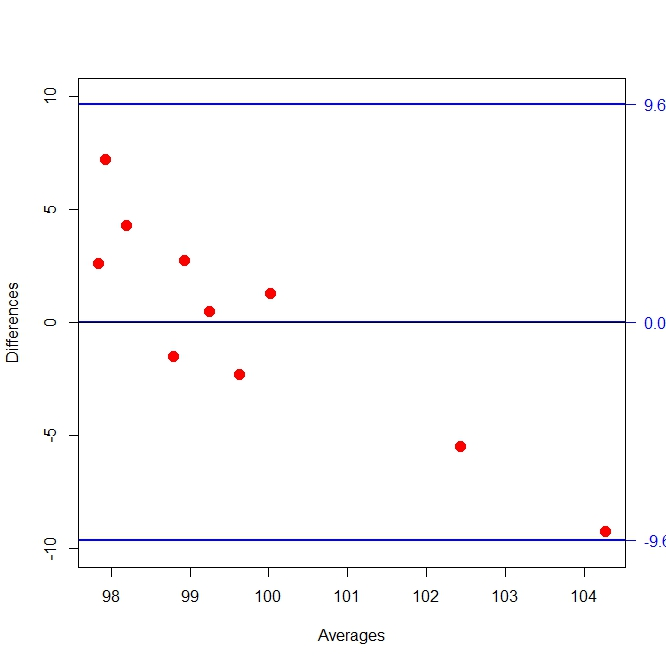
\includegraphics[width=0.7\linewidth]{images/EAD1}
	\caption{Expected Absolute Difference}
	\label{fig:EAD1}
\end{figure}

\citet{Barnhart} remarks that a comparison of EAD and MSD , using
simulation studies, would be interesting, while further adding
that `\textit{It will be of interest to investigate the benefits of these
	possible new unscaled agreement indices}'. For the Grubbs' `F vs C' and `F vs T' comparisons, the inter-method bias, difference variances, limits of agreement and EADs are shown
in Table 1.5. The corresponding Bland-Altman plots for `F vs C' and `F vs T' comparisons were depicted previously on Figure 1.3. While the inter-method bias for the `F vs T' comparison is smaller, the EAD penalizes the comparison for having a greater variance of differences. Hence the EAD values for both comparisons are much closer.
\begin{table}[ht]
	\begin{center}
		\begin{tabular}{|c|c|c|}
			\hline
			& F vs C & F vs T  \\
			\hline
			Inter-method bias & -0.61 & 0.12 \\
			Difference variance & 0.06 & 0.22  \\
			Limits of agreement & (-1.08,	-0.13) & (-0.81,1.04) \\
			EAD & 0.61 & 0.35  \\
			\hline
		\end{tabular}
		\caption{Agreement indices for Grubbs' data comparisons.}
	\end{center}
\end{table}

Further to  \citet{lin2000} and \citet{lin2002}, individual agreement between two measurement methods may be
assessed using the the coverage probability (CP) criteria or the total deviation index (TDI). If $d_{0}$ is predetermined as the maximum acceptable absolute difference between two methods of measurement, the probability that the absolute difference of two measures being less than $d_{0}$ can be computed. This is known as the coverage probability (CP).

\begin{equation}
CP = P(|x_{i} - y_{i}| \leq d_{0})
\end{equation}

If $\pi_{0}$ is set as the predetermined coverage probability, the
boundary under which the proportion of absolute differences is
$\pi_{0}$ may be determined. This boundary is known as the `total
deviation index' (TDI). Hence the TDI is the $100\pi_{0}$
percentile of the absolute difference of paired observations.


\section*{Coverage Probability and Total Deviation Index}
% Barnhart

As elaborated by Lin and colleagues (Lin, 2000; Lin et al., 2002), an intuitive measure of
agreement is a measure that captures a large proportion of data within a boundary for allowed
observers’ differences. The proportion and boundary are two quantities that correspond to
each other. If we set d0 as the predetermined boundary; i.e., the maximum acceptable
absolute difference between two observers’ readings, we can compute the probability of absolute
difference between any two observers’ readings less than d0. 

%This probability is called coverage probability (CP). On the other hand, if we set 0 as the predetermined coverage probability, we can find the boundary so that the probability of absolute difference less than this boundary is 0. This boundary is called total deviation index (TDI) and is the 1000 percentile of the absolute difference of paired observations. A satisfactory agreement may require a large CP or, equivalently, a small TDI.

%For J = 2 observers, let Yi1 and Yi2 be the
%readings of these two observers, the CP and TDI are defined as
%\[
%CPd0 = Prob(|Yi1 − Yi2| < d0), TDI0 = f−1(0)
%\]
%where f−1(0) is the solution of d by setting $f(d) = Prob(|Yi1 − Yi2| < d) = 0$.
%Estimation and inference on CPd0 and TDI0 often requires a normality assumption on
%Di = Yi1 − Yi2.Assume that Di is normally distributed with mean μD and variance 2
%D .


	
	\section*{Coverage probability (CP)}
	Another user friendly measure of agreement which is related to the computation of the TDI is the so called coverage probability (CP) [11,12]. 
	The CP describes the proportion captured within a pre-specified boundary of the absolute paired-measurement differences from two devices, i.e., the value of p$\kappa$ such that $P(|D| < \kappa$) = $p_\kappa$. Therefore one can find p$\kappa$ for a specified boundary $\kappa$ using standard methods for computing probability quantities under normal assumptions [11]:
	
	(13)
	and to obtain a CP estimate, p$\kappa$ can be computed by replacing $\mu_D$ and $\sigma_D$ by their REML estimate counterparts derived from model (1).
	
	As with the TDI, the CP criterion can also be translated into a hypothesis test specification. 
	In this case the interest is to ensure that a specified boundary of the absolute paired-measurement differences captures at least a predetermined proportion, p0:
	
	
	The proposed TI method for inference about the TDI can be utilized to perform inferences about the CP estimates. From the TI in (10) it follows that
	
	(14)
	Now $\kappa$ is a fixed known boundary, and our interest lies in finding a lower confidence bound for the CP estimate. 
	Thus, one can find a lower confidence bound for a non-central Student-t proportion with confidence level 1 - $\alpha$ by searching the non-centrality parameter, 
	that depends on  and hence on p$\kappa$, that satisfies
	
	(15)
	and once the non-centrality parameter  is achieved, a lower bound about the proportion p$\kappa$ is found using equation (5), 
	
	% p$\kappa$ = Φ() - Φ(-2μD/σD - ).
	
	However, the non-centrality parameter cannot be found in a closed form, so one may use again a modified version of the binary search algorithm as follows:
	
	\begin{enumerate}
		\item begin with the interval [low = 0; high = 1], as p$\kappa$ is bounded by the interval (0,1);
		
		\item calculate the midpoint of the interval \textit{mid = (low + high)/2} and compute the difference ;
		
		\item if d is greater than 0 up to a tolerance bound $\delta$ (i.e., ), then recalculate the interval [low = mid + $\delta$; high = 1]; if it is 
		lower than 0 up to a tolerance bound $\delta$ (i.e. ), then recalculate the interval [low = 0; high = mid - $\delta$];
		
		\item repeat steps 2-3 until convergence, i.e. until d satisfies .
	\end{enumerate}
\newpage
\section{Probability-based Measures of Agreement}
There are two measures of agreement based on the probability criteria. The first is the
$p_0$-th percentile of jDj, say Q($p_0$), where $p_0$ (> 0.5) is a specified large probability (usually ¸ 0:80). 
It was introduced by Lin (2000) who called it the total deviation index (TDI). Its
small value indicates a good agreement between (X; Y ). The TDI can be expressed as,

! EQUATION HERE
-distribution with a single degree of freedom and non-centrality parameter \textbf{\textit{Del}}.

%-----------------------------------------------------------------------------------------%
%Coverarge Probability

The second measure, introduced by Lin et al. (2002), is the \textbf{coverage probability} (CP) of
the interval [¡±0; ±0], where a difference under §±0 is considered practically equivalent to
zero. There is no loss of generality in taking this interval to be symmetric around zero as it
can be achieved by a location shift. 

Letting,
dl = (¡±0 ¡ ¹)=¾; du = (±0 ¡ ¹)=¾; (2)


the CP can be expressed as
F(±0) = ©(du) ¡ ©(dl): (3)

A high value of F(±0) implies a good agreement between the methods.


\section*{Total Deviation Index}



Total deviation index for measuring individual agreement with applications in laboratory performance and bioequivalence.
Lin LI.
*Stat Med. 2000 Jan 30;19(2):255-70*
*http://www.ncbi.nlm.nih.gov/pubmed/10641028*




%%====================%%
In areas of inter-laboratory quality control, method comparisons, assay validation and individual bioequivalence, etc., the agreement between observations and target (reference) values is of interest. The mean of the squared difference between observations and target values (MSD) is a good measure of the total deviation. A new user-friendly statistic, the total deviation index (TDI(1-p)), is introduced that translates the MSD into an index that can be directly compared to a predetermined criterion. 

\bigskip 

The TDI(1-p) describes a boundary such that a majority, 100(1-p) per cent, of the observations are within the boundary (measurement unit and/or per cent) from their target values. Statistical inference using the sample counter part (estimate) is presented. A Monte Carlo experiment with 5000 runs was performed to confirm the estimate's validity. Applications in laboratory performance and validation, as well as individual bioequivalence, are presented.
%%====================%%
%- http://www.tandfonline.com/doi/abs/10.1080/10543400802622576#.U5f-GnJdXw0
%- 

\bigskip

Individual agreement between two measurement systems is determined using the total deviation index (TDI) or the coverage probability (CP) criteria as proposed by Lin (2000) and Lin et al. (2002). We used a variance component model as proposed by Choudhary (2007). Using the bootstrap approach, Choudhary (2007), and generalized confidence intervals, we construct bounds on TDI and CP. A simulation study was conducted to assess whether the bounds maintain the stated type I error probability of the test. We also present a computational example to demonstrate the statistical methods described in the paper.

%%====================%%
- http://artax.karlin.mff.cuni.cz/r-help/library/MethComp/html/TDI.html

	
	\section{Coverage Probability and Tolerance Deviation Index}

	The CP is the most intuitively clear approach; it mirrors the information provided by the TDI. 
	Both TDI and CP depend on the normality assumption and offer better power
	for inference than the CCC. The CP would have difŽficulty discriminating among instruments or 
	assays that have excellent agreement, all because the CP values would be very close to
	1. In this case, the TDI can be used to discriminate among these. When a meaningful clinical range is known and the study is conducted over that range, the CCC offers a meaningful geo- metric interpretation and is unit free. Furthermore, the accuracy and precision components of the CCC offer more insight. Therefore, the CCC, accuracy, and precision remain very useful tools. Note that when Y and X are not linearly related, the CCC will capture the total deviation. However, it will treat the nonlinear deviation as imprecision rather than inaccuracy. The CCC, ICC, and Pearson correlation coefŽ cient depend
	largely on the analytical range and the intrasample variation.
	


	
\section{Total Deviation Index and Coverage Probability}
%------------------------------------------------------------------------------%
	
	%http://statistics.unl.edu/faculty/yang/agreement.pdf
	%http://www.biomedcentral.com/content/pdf/1471-2288-10-31.pdf

%------------------------------------------------------------------------------%

\citet{lin2002} proposes a measure called the `Total Deviation Index'. 
This assumes that the differences of paired measurements are a random sample from a normal distribution, and consequently the approach is to construct a probability interval, known as a tolerance interval, for these differences. A tolerance interval is a statistical range within which a specified proportion of the population lies.

%------------------------------------------------------------------------------%

Smaller values of $q$ indicate better agreement. $P_{0}$ is specified by the practitioner.
	
\citet{pkcng} generalize this approach to account for situations where the distributions are not identical, which is commonly the case.
	The TDI is not consistent and may not preserve its asymptotic nominal level, and that the coverage probability approach of \citet{lin2002} is overly conservative for moderate sample sizes.
	This methodology proposed by \citet{pkcng} is a regression based approach that models the mean and the variance of differences as functions of observed values of the average of the paired measurements.
	These methodologies have been adopted by Mayo Clinic (Research Section).
	
	% Link: http://mayoresearch.mayo.edu/mayo/research/biostat/sasmacros.cfm
	
	%------------------------------------------------------------------------------%
	This measure was coined by Lin as the value \[TDI_{1-p} = \kappa\] that a given fraction (1-p) of the differences between two measurement methods will be in a symmetric interval $[-\kappa,\kappa]$.
	This is roughly equivalently to the numerically largest of the 1-p limits of agreement.
	The measure clearly has its main applicability in equivalence testing. 
	
	Lin gives an approximate formula for the calculations.
	\[\Theta \left( \frac{ TDI - \mu_d}{\sigma_d} \right) - \Theta \left(  \frac{ -TDI - \mu_d}{\sigma_d} \right) = 1-p\]
	
	Again, the assumption of the normality of the case-wise differences is relied upon.
	
\section*{Total Deviation Index - TDI - Escaramis}


%% Website
%%http://www.biomedcentral.com/1471-2288/10/31/

%% Paper
The Total Deviation Index estimated by Tolerance Intervals to evaluate the concordance of measurement devices.  
Geòrgia Escaramís1, Carlos Ascaso1 and Josep L Carrasco1.  

%% Background
In an agreement assay, it is of interest to evaluate the degree of agreement between the different methods (devices, instruments or observers) used to measure the same characteristic. We propose in this study a technical simplification for inference about the total deviation index (TDI) estimate to assess agreement between two devices of normally-distributed measurements and describe its utility to evaluate inter- and intra-rater agreement if more than one reading per subject is available for each device.

%%###Methods
We propose to estimate the TDI by constructing a probability interval of the difference in paired measurements between devices, and thereafter, we derive a tolerance interval (TI) procedure as a natural way to make inferences about probability limit estimates. We also describe how the proposed method can be used to compute bounds of the coverage probability.

%%###Results
The approach is illustrated in a real case example where the agreement between two instruments, a handle mercury sphygmomanometer device and an OMRON 711 automatic device, is assessed in a sample of 384 subjects where measures of systolic blood pressure were taken twice by each device. A simulation study procedure is implemented to evaluate and compare the accuracy of the approach to two already established methods, showing that the TI approximation produces accurate empirical confidence levels which are reasonably close to the nominal confidence level.

%%%Conclusions
The method proposed is straightforward since the TDI estimate is derived directly from a probability interval of a normally-distributed variable in its original scale, without further transformations. Thereafter, a natural way of making inferences about this estimate is to derive the appropriate TI. Constructions of TI based on normal populations are implemented in most standard statistical packages, thus making it simpler for any practitioner to implement our proposal to assess agreement.
\newpage
	

	
	\section{Total Deviation Index and Coverage Probability}
	%------------------------------------------------------------------------------%
	
	%http://statistics.unl.edu/faculty/yang/agreement.pdf
	%http://www.biomedcentral.com/content/pdf/1471-2288-10-31.pdf
	%------------------------------------------------------------------------------%
	
	\citet{lin2002} proposes a measure called the `Total Deviation Index'. 
	This assumes that the differences of paired measurements are a random sample from a normal distribution, 
	and consequently the approach is to construct a probability interval, known as a tolerance interval, 
	for these differences. A tolerance interval is a statistical range within which a specified proportion 
	of the population lies.
	%------------------------------------------------------------------------------%
	Smaller values of $q$ indicate better agreement. $P_{0}$ is specified by the practitioner.
	
	\citet{pkcng} generalize this approach to account for situations where the distributions are not identical, which is commonly the case.
	The TDI is not consistent and may not preserve its asymptotic nominal level, and that the coverage probability approach of \citet{lin2002} is overly conservative for moderate sample sizes.
	This methodology proposed by \citet{pkcng} is a regression based approach that models the mean and the variance of differences as functions of observed values of the average of the paired measurements.
	These methodologies have been adopted by Mayo Clinic (Research Section).
	
	% Link: http://mayoresearch.mayo.edu/mayo/research/biostat/sasmacros.cfm
	
	
	
	\section{Unscaled Agreement Indices}
	\begin{itemize}
		\item Summary agreement indices based on the absolute difference of readings by observers are
		grouped here as unscaled agreement indices. 
		\item They are usually defined as the expectation
		of a function of the difference, or features of the distribution of the absolute difference.
		
		\item
		These indices include mean squared deviation, repeatability coefficient, repeatability variance,
		reproducibility variance (ISO), limits of agreement (Bland and Altman, 1999), coverage
		probability (CP) and total deviation index (TDI) (Lin et al., 2002 Choudhary and Nagaraja,
		2007; Choudhary, 2007a).
	\end{itemize}
	
	
	% Assessment of disagreement: a new information-based approach
	% C Costa-Santos, L Antunes, A Souto, J Bernardes - Annals of epidemiology, 2010 - Elsevier
	%---------------------------------------------------------------------------------%
	\section{Information Approach}
	
	PURPOSE: Disagreement on the interpretation of diagnostic tests and clinical decisions 
	remains an important problem in medicine. As no strategy to assess agreement seems to be 
	fail-safe to compare the degree of agreement, or disagreement, 
	
	
	%---------------------------------------------------------------------------------%
	
	\subsection{Example: Systolic Blood Pressure}
	Bland and Altman (19) present the example of measurements of systolic blood pressure of 85 individuals, by two observers (observer J and observer R) with sphygmomanometer, and one other measurement, by a semiautomatic device (device S). Luiz et al. (16) re-analyze the data and also observe, with a graphical approach, a greater agreement between the two observers than between the observers and the semiautomatic device. Using our information-based measure of disagreement; we also obtained a significantly more
	disagreement between each observer and the semiautomatic device than between the two observers (Table 1).
	
	%---------------------------------------------------------------------------------%
	
	\subsection{Discussion}
	
	\begin{itemize}
		\item We can look at disagreement between observers as the distance between their ratings, so the metric properties are important. Moreover, the proposed measure of disagreement is scale-invariant, i.e., the degree of disagreement between two observers should be the same if the measurements are analyzed in kilograms or in grams, for example.
		
		\item Differential weighting is another property of the proposed information-based measure of disagreement: each comparison between two ratings is divided by a normalizing factor, depending on each pair of ratings alone, before summing. Therefore, the information-based measure of disagreement is appropriate for ratio scale measurements (with a natural 0) and it is not appropriate for interval scale measurements (without a natural 0). 
		
		\item For example, outside air temperature in Celsius (or Fahrenheit) scale does not have a natural 0. The 0° is arbitrary and it does not make sense to say that 20° is twice as hot as 10°. Outside air temperature in Celsius (or Fahrenheit) scale is an interval scale. On the other hand, height has a natural 0 meaning: the absence of height. Therefore, it makes sense to say that 80 inches is twice as large as 40 inches. Height is a ratio scale. 
		
		\item Suppose the heights of a sample of subjects measured independently by two different observers. A difference between the two observers of 1 inch in a child subject represents a worse observers' error than a disagreement between observers of 1 inch in an adult subject. 
		
		\item Due to differential weighting property of the information-based measure of disagreement, a difference between the observers of one inch in a child in fact weights less to the estimate of information-based measure of disagreement between observers than a difference between the observers of 1 inch in an adult.
		
		\item The usual approaches used to evaluate agreement have the limitation of the comparability of populations. In fact, ICC depends on the variance of the trait in the population; although this characteristic can be considered an advantage it does not permit one to compare the degree of agreement across different populations. Also the interpretation of the limits of agreement depends on what can be considered clinically relevant or not, which could be subjective and different from reader to reader. 
		
		\item The comparison of the degree of agreement in different populations is not straightforward. Other approaches 16 and 17 to assess observer agreement have been proposed, however the comparability of populations is still not easy with these approaches.
		
		\item The proposed information-based measure of disagreement, used as a complement to current approaches for evaluating agreement, can be useful to compare the degree of disagreement among different populations with different characteristics, namely with different variances.
		
		\item Moreover, we believe that information theory can make an important contribution to the relevant problem of measuring agreement in medical research, providing not only better quantification but also better understanding of the complexity of the underlying problems related to the measurement of disagreement.
	\end{itemize}
	
	
	%CoverageProbability
	
	\subsection{Coverage probability}
	This term refers to the probability that a procedure for 
	constructing random regions will produce an interval containing, or covering, the 
	true value. It is a property of the interval producing procedure, and is 
	independent of the particular sample to which such a procedure is applied. We 
	can think of this quantity as the chance that the interval constructed by such a 
	procedure will contain the parameter of interest.
	
	% http://en.wikipedia.org/wiki/Coverage_probability
	% http://www.stats.ox.ac.uk/pub/bdr/IAUL/Course1Notes5.pdf
	

	
	
	
	\section{LME - Pankaj Choudhury}
	Consistent with the conventions of mixed models, \citep{pkc}
	formulates the measurement $y_{ij} $from method $i$ on individual
	$j$ as follows;
	\begin{equation}
	y_{ij} =P_{ij}\theta + W_{ij}v_{i} + X_{ij}b_{j} + Z_{ij}u_{j} +
	\epsilon_{ij},     (j=1,2, i=1,2....n)
	\end{equation}
	The design matrix $P_{ij}$ , with its associated column vector
	$\theta$, specifies the fixed effects common to both methods. The
	fixed effect specific to the $j$th method is articulated by the
	design matrix $W_{ij}$ and its column vector $v_{i}$. The random
	effects common to both methods is specified in the design matrix
	$X_{ij}$, with vector $b_{j}$ whereas the random effects specific
	to the $i$th subject by the $j$th method is expressed by $Z_{ij}$,
	and vector $u_{j}$. Noticeably this notation is not consistent
	with that described previously.  The design matrices are specified
	so as to includes a fixed intercept for each method, and a random
	intercept for each individual. Additional assumptions must also be
	specified;
	\begin{equation}
	v_{ij} \sim N(0,\Sigma),
	\end{equation}
	These vectors are assumed to be independent for different $i$s,
	and are also mutually independent. All Covariance matrices are
	positive definite.  In the above model effects can be classed as
	those common to both methods, and those that vary with method.
	When considering differences, the effects common to both
	effectively cancel each other out. The differences of each pair of
	measurements can be specified as following;
	\begin{equation}
	d_{ij} = X_{ij}b_{j} + Z_{ij}u_{j} + \epsilon_{ij},     (j=1,2,
	i=1,2....n)
	\end{equation}
	This formulation has seperate distributional assumption from the
	model stated previously.
	
	This agreement covariate $x$ is the key step in how this
	methodology assesses agreement.
	
	\citet{pkcng} generalize this approach to account for situations
	where the distributions are not identical, which is commonly the
	case. The TDI is not consistent and may not preserve its
	asymptotic nominal level, and that the coverage probability
	approach of \citet{lin2002} is overly conservative for moderate
	sample sizes. This methodology proposed by \citet{pkcng} is a
	regression based approach that models the mean and the variance of
	differences as functions of observed values of the average of the
	paired measurements.

\addcontentsline{toc}{section}{Bibliography}

%--------------------------------------------------------------------------------------%

\bibliographystyle{chicago}
\bibliography{DB-txfrbib}
\end{document}
